\chapter{Test pictures}
\section{Delopgave 2}
\begin{figure}[h!]
\centering
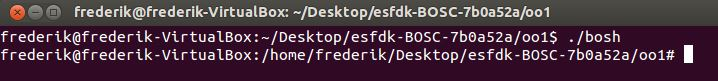
\includegraphics{Images/TestOfPart2}
\label{Test2}
\end{figure}

\section{Delopgave 3}
\begin{figure}[h!]
\centering
\caption{Test 1}
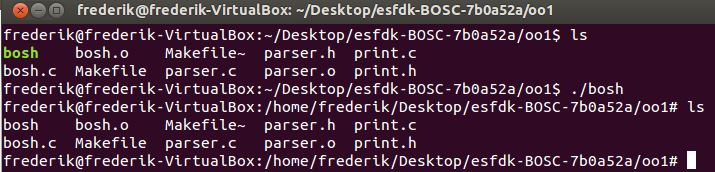
\includegraphics{Images/TestOfPart3_1}
\label{Test3_1}
\end{figure}

\begin{figure}[h!]
\centering
\caption{Test 2}
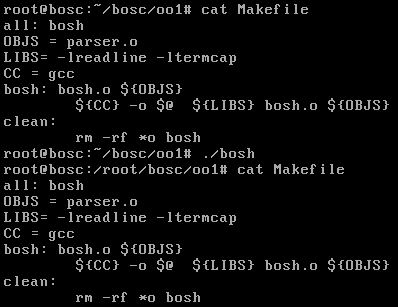
\includegraphics{Images/TestOfPart3_2}
\label{Test3_2}
\end{figure}

\begin{figure}[h!]
\centering
\caption{Test 3}
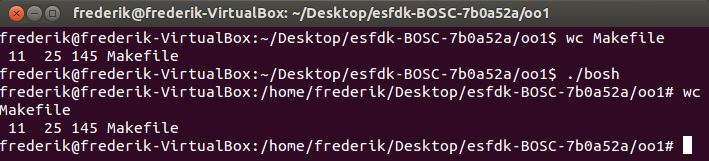
\includegraphics{Images/TestOfPart3_3}
\label{Test3_3}
\end{figure}

\begin{figure}[!ht]
\centering
\caption{Test 4}
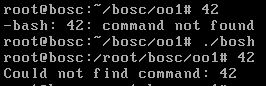
\includegraphics{Images/TestOfPart3_4}
\label{Test3_4}
\end{figure}

\clearpage
\section{Delopgave 4}
\begin{figure}[!h]
\centering
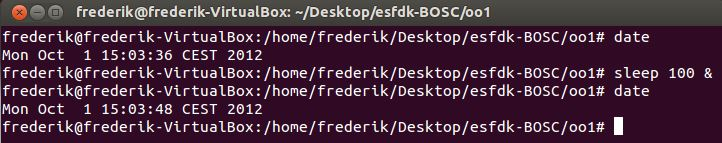
\includegraphics{Images/TestOfPart4}
\label{Test4}
\end{figure}

\section{Delopgave 5}
\begin{figure}[!h]
\centering
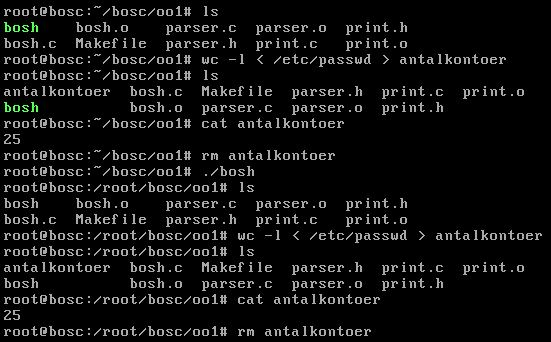
\includegraphics{Images/TestOfPart5}
\label{Test5}
\end{figure}

\section{Delopgave 6}
\begin{figure}[!h]
\centering
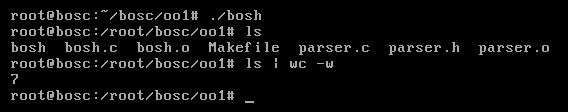
\includegraphics{Images/TestOfPart6}
\label{Test6}
\end{figure}

\section{Delopgave 7}
\begin{figure}[!h]
\centering
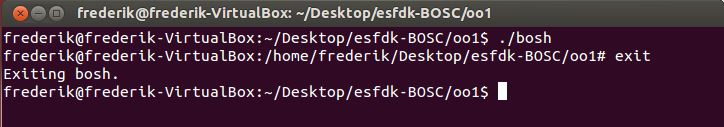
\includegraphics{Images/TestOfPart7}
\label{Test7}
\end{figure}

\section{Delopgave 8}
\begin{figure}[!h]
\centering
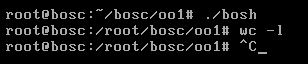
\includegraphics{Images/TestOfPart8}
\label{Test8}
\end{figure}

\section{Ekstrafunktionalitet 1}
\begin{figure}[!h]
\centering
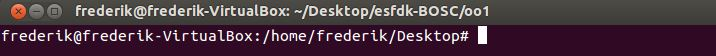
\includegraphics{Images/TestOfPart9}
\label{Test9}
\end{figure}

\section{Ekstrafunktionalitet 2}
\begin{figure}[!h]
\centering
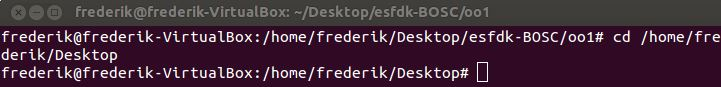
\includegraphics{Images/TestOfPart10}
\label{Test10}
\end{figure}